\chapter{Example Chapter for the Thesis}

\section{Abstract}
Here's an example of an abstract for your chapter.

\section{Introduction}
Here's an introduction. There is also a picture of a chicken (Fig. \ref{fig:chicken}).

\begin{figure}
	\centering
	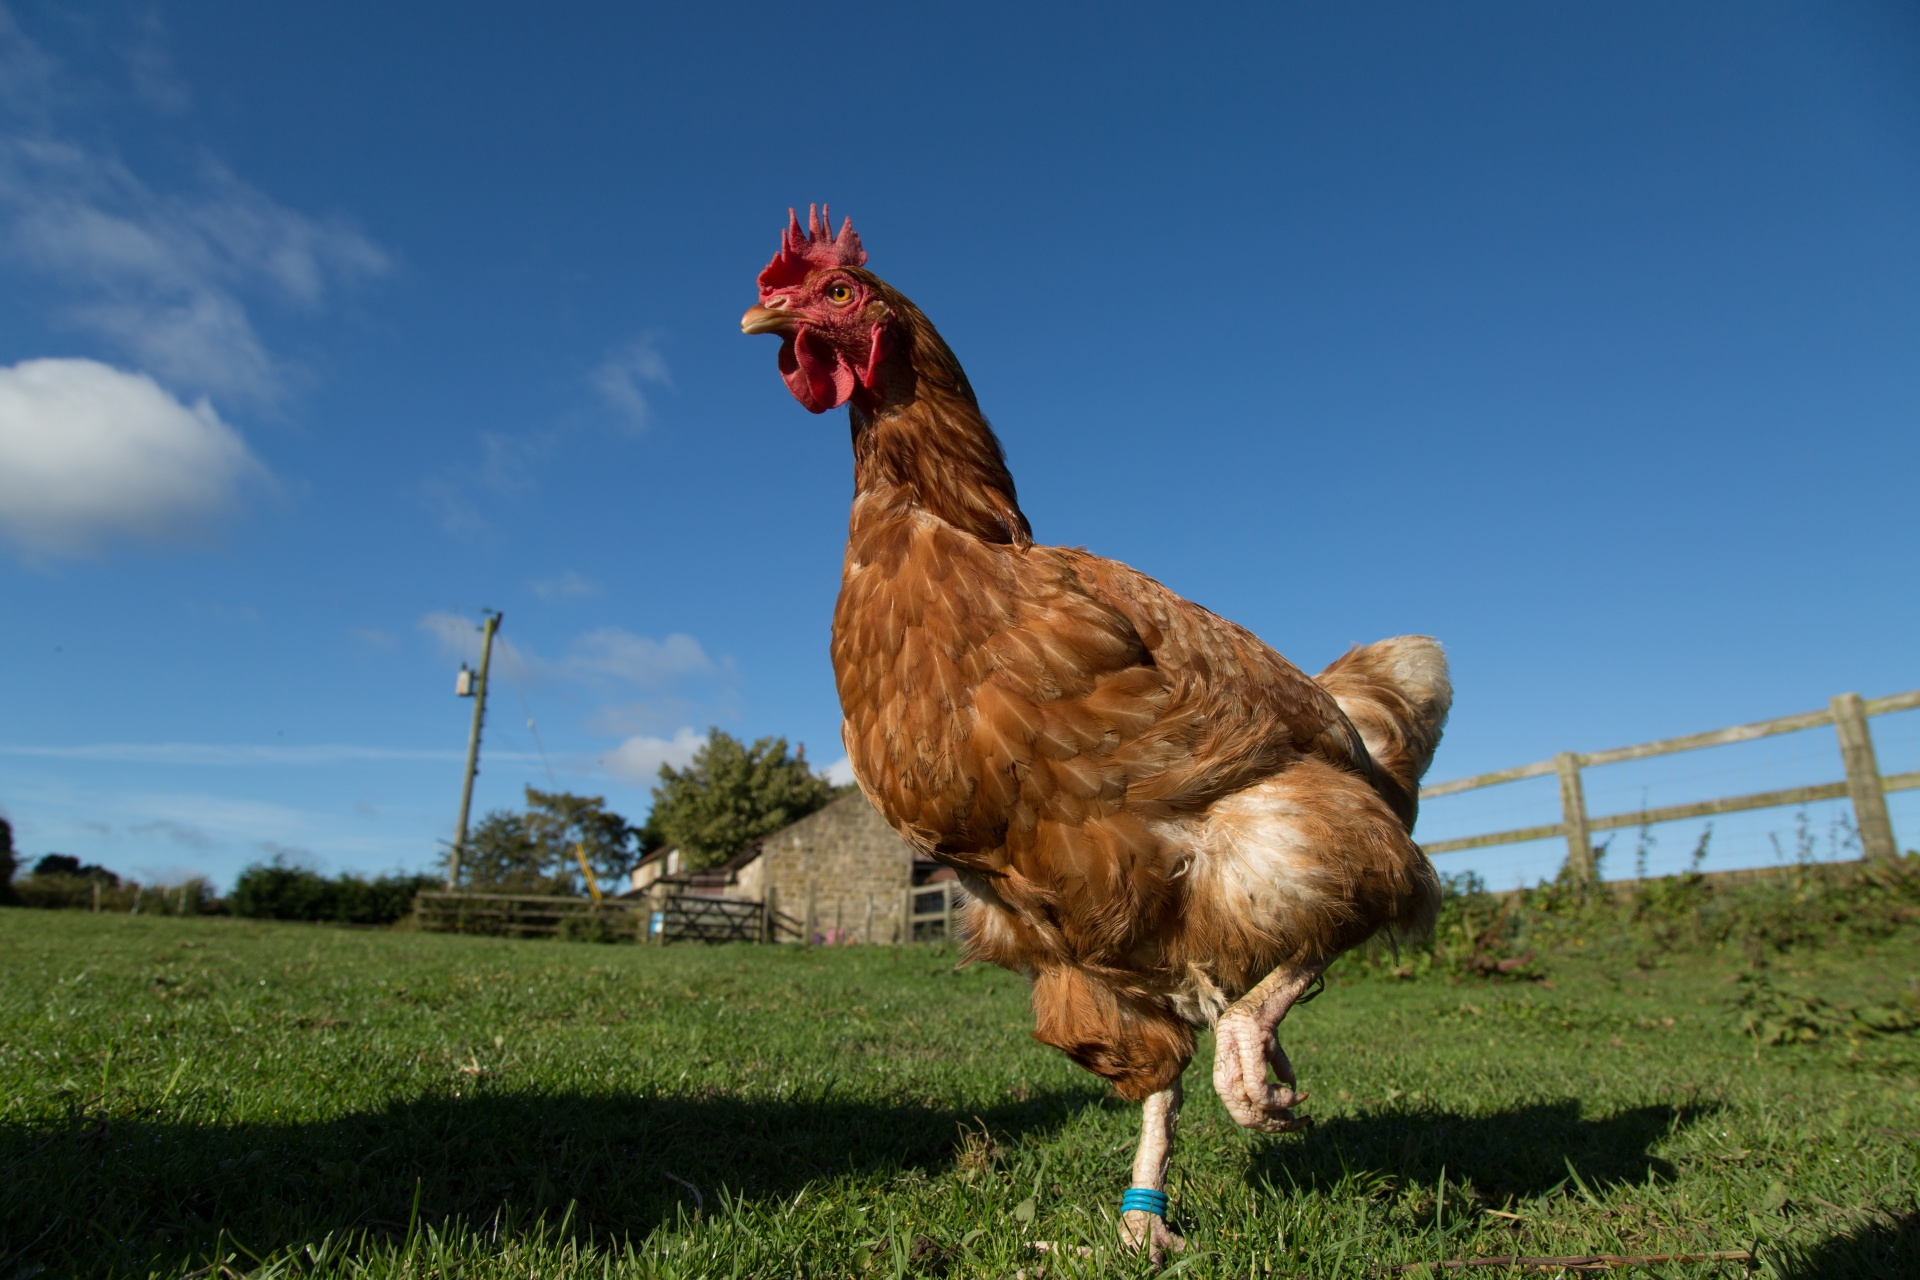
\includegraphics[width=0.5\textwidth]{chicken.jpg} % common domain
	\caption{This is a chicken.}
	\label{fig:chicken}
\end{figure}


\section{Methods}
Here's another section.

\subsection{Data}
Here's a subsection. We can cite things for these sentences easily \parencite{cadotte_should_2017,del-rio_birds_2021}.

\begin{equation}\label{eqn}
	a^2 + b^2 = c^2
\end{equation}

\section{More information}
See something in \hyperref[appendix:ch1]{Appendix A}. \textbf{NOTE} in the code document that I had to use `hyperref` and not `ref` for the appendix.